\section{Adaptive Step Sizes}

\begin{enumerate}[label=\alph*), leftmargin=*]

%% a)
\item
%

Let a Moving Average process $x(n)$ of order $q=1$, MA(1), such that:

\begin{equation}
    x(n) = 0.9 \eta(n - 1) + \eta(n), \quad \eta \sim \mathcal{N}(0, 0.5)
\end{equation}

When LMS is used with a constant step-size $\mu$, a trade-off between convergence speed, smoothness and oscillations magnitude at steady-state is inevitable.
Gradient Adaptive Step-Size (GASS) algorithms attempt to combine the positive aspects of both
large and small values of $\mu$ by adapting its magnitude according to the gradient $\nabla_{\mu} \mathcal{J}$, where $\mathcal{J}$ the objective function
minimised by the adaptive filter.

Different GASS algorithms, namely Benvenist, Ang \& Farhan and Matthews \& Xi, are implemented and their performance is compared to simple constant step-size LMS algorithm.
Weight error and squared prediction error curves are provided at figure \ref{fig:3_2_a}.

\begin{figure}[h]
    \centering
    \begin{subfigure}{0.49\textwidth}
        \centering
        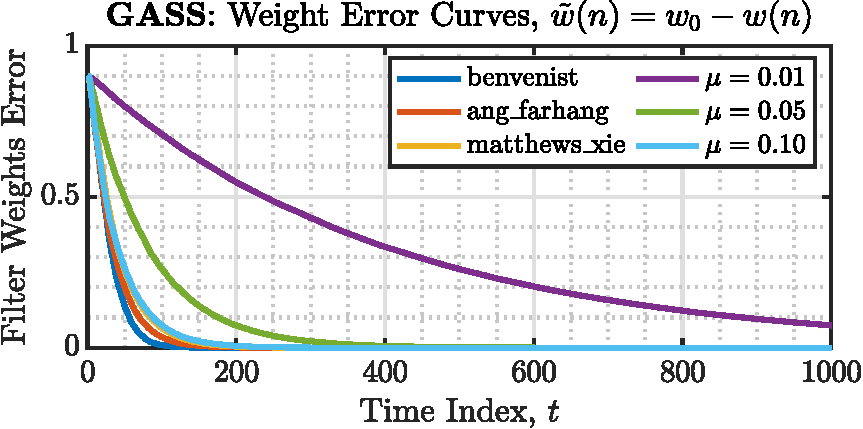
\includegraphics[height=1.5in]{report/adaptive-signal-processing/adaptive-step-sizes/assets/a/weight_error_curves}
    \end{subfigure}
    ~
    \begin{subfigure}{0.49\textwidth}
        \centering
        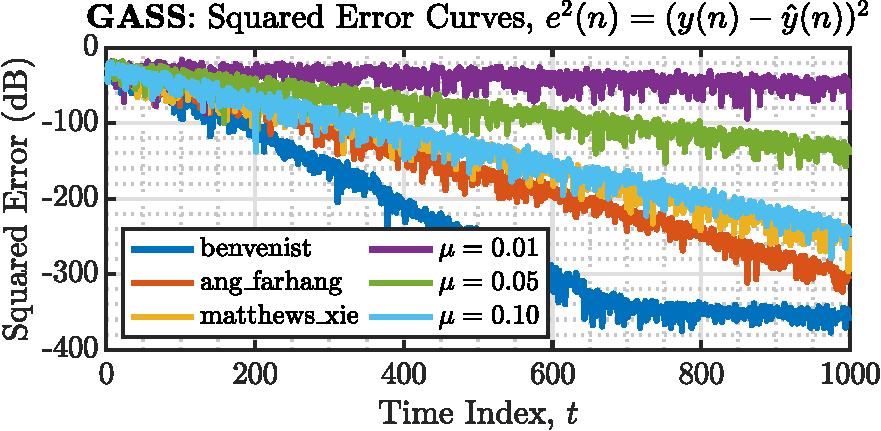
\includegraphics[height=1.5in]{report/adaptive-signal-processing/adaptive-step-sizes/assets/a/squared_prediction_error}
    \end{subfigure}
    \caption{GASS LMS: weight error and squared prediction error curves.}
    \label{fig:3_2_a}
\end{figure}

All GASS algorithms converge to the true process parameters faster than simple LMS (within less than 50 steps), while unsurprisingly,
the most computationally intensive algorithm, Benvenist ($\mathcal{O}(M^{2})$), adapts first of all and scores the smallest squared prediction error.
Moreover, their steady-state error is much smaller (below $-300dB$) than the fixed step-size LMS algorithm (at $-200dB,\ -120dB,\ -30dB$ for $\mu = 0.1,\ 0.05,\ 0.01$, respectively),
improving the EMSE from the previous part.

%% b)
\item
%

Starting from the update equation based on the \textit{a posteriori error} $e_{p}(n) = d(n) - \mathbf{x}(n)^{T} \vw(n + 1)$:

\begin{equation}
    \vw(n + 1) = \vw(n) + \mu e_{p}(n) \mathbf{x}(n)
\label{eq:nlms_a_error}
\end{equation}

Multiply both sides with $-\mathbf{x}(n)^{T}$ and add $d(n)$ to construct $e_{p}(n)$ on the LHS:

\begin{equation}
    d(n) - \mathbf{x}(n)^{T} \vw(n + 1) = d(n) - \mathbf{x}(n)^{T} \vw(n) - \mathbf{x}(n)^{T} \mu e_{p}(n) \mathbf{x}(n)
\end{equation}

Note that the LHS term is the a posteriori error, $e_{p}(n)$, while the first RHS term the a priori error, $e(n)$:

\begin{align}
    e_{p}(n)    &= e(n) - \mu e_{p}(n) \| \mathbf{x}(n) \|^{2} \\
    e_{p}(n)    &= e(n) \frac{1}{1 + \mu \| \mathbf{x}(n) \|^{2}}
                % &= e(n) \bigg[ \frac{1 + \mu \| \mathbf{x}(n) \|^{2} - \mu \| \mathbf{x}(n) \|^{2} }{1 + \mu \| \mathbf{x}(n) \|^{2}} \bigg] \\
                % &= e(n) \bigg[ 1 - \mu \frac{\| \mathbf{x}(n) \|^{2}}{1 + \mu \| \mathbf{x}(n) \|^{2}} \bigg]
\label{eq:aa_errors}
\end{align}

Substituting (\ref{eq:aa_errors}) in update equation (\ref{eq:nlms_a_error}):

\begin{align}
    \vw(n + 1)  &= \vw(n) + \mu \frac{1}{1 + \mu \| \mathbf{x}(n) \|^{2}} e(n) \mathbf{x}(n) \\
    \vw(n + 1)  &= \vw(n) + \frac{1}{\frac{1}{\mu} + \| \mathbf{x}(n) \|^{2}} e(n) \mathbf{x}(n) \\
    \vw(n + 1)  &= \vw(n) + \frac{\beta}{\epsilon + \| \mathbf{x}(n) \|^{2}} e(n) \mathbf{x}(n) \label{eq:nlms}
\end{align}

where for $\beta = 1$ and $\epsilon = \frac{1}{\mu}$ we showed that the NLMS update (\ref{eq:nlms}) is equivalent to the update equation based on the \textit{a posteriori error},
given by (\ref{eq:nlms_a_error}).

%% c)
\item
%

The implementation of Generalized Nnormalized Gradient Descent (GNGD) algorithm is compared with the the Benvenist GASS algorithm, and the weight error and squared prediction error curves
are provided at figure \ref{fig:3_2_c}. We notice that the GNGD algorithm converges to the true process parameters within 30 timesteps,
faster than the Benvenist GASS algorithm which reaches a steady-state in 50 timesteps. This is also reflected in the squared prediction error curves,
where the GNGD error is always smaller than the Benvenist GASS prediction error.

\begin{figure}[h]
    \centering
    \begin{subfigure}{0.49\textwidth}
        \centering
        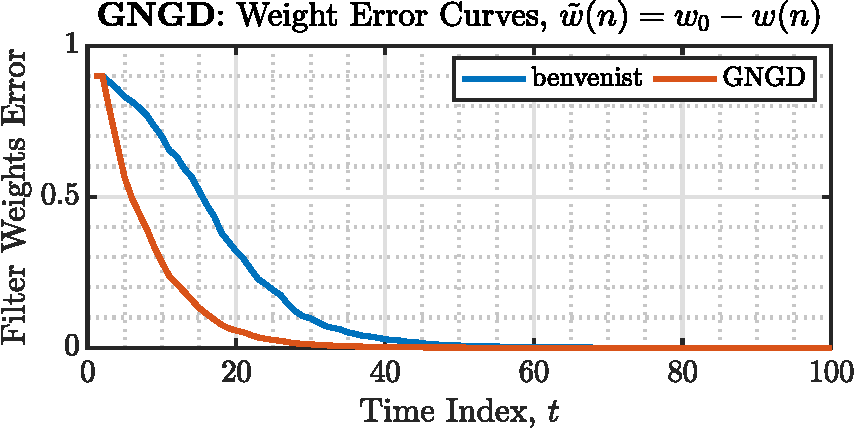
\includegraphics[height=1.5in]{report/adaptive-signal-processing/adaptive-step-sizes/assets/c/weight_error_curves}
    \end{subfigure}
    ~
    \begin{subfigure}{0.49\textwidth}
        \centering
        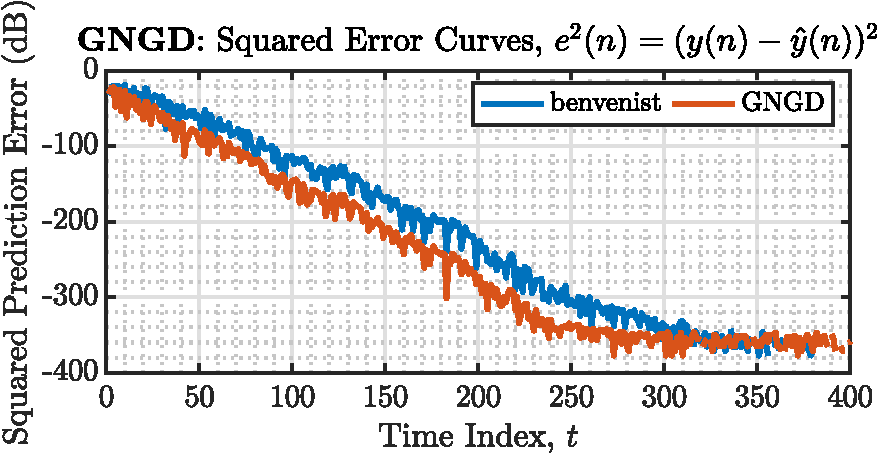
\includegraphics[height=1.5in]{report/adaptive-signal-processing/adaptive-step-sizes/assets/c/squared_prediction_error}
    \end{subfigure}
    \caption{GNGD vs Benvenist GASS: weight error and squared prediction error curves.}
    \label{fig:3_2_c}
\end{figure}

In the previous part we empirically showed the superiority of the Benvenist GASS algorithm over the other GASS algorithms and the standard LMS, in terms of performance (speed \& prediction error).
Nonetheless, this improved performance comes with an increased computational complexity load.

Let $M$ the model order (number of lags in MA or AR model process), then the input vector $\mathbf{x}(n) \in \sR^{M}$.

Each update of the Benvenist GASS algorithm involves the calculation of 
\begin{itemize}
    \item the outer product $\mathbf{x}(n-1) \mathbf{x}(n-1)^{T}$
    \item the matrix product $\big[I - \mu(n-1) \mathbf{x}(n-1) \mathbf{x}(n-1)^{T} \big] \boldsymbol{\psi}(n - 1)$
\end{itemize}

which both have quadratic complexity in $M$. Hence Benvenist GASS algorithm is $\mathbf{\mathcal{O}(M^{2})}$.

Each update of the GNGD algorithm involves only inner product calculations, additions of $M$-dimensional vectors and scalar operations, all bounded by linear complexity in $M$.
Therefore, GNGD algorithm is $\mathbf{\mathcal{O}(M)}$.

Surprisingly, the GNGD algorithm does not only perform better (convergence speed and prediction error) than the Benvenist GASS algorithm, but it is also computationally less expensive.

%
\end{enumerate}